\section{Funzioni}

\begin{frame}[fragile]
\frametitle{Funzioni}
    \begin{block}{}
        \begin{itemize}
            \item Abbiamo già visto e usato alcune funzioni, ad esempio: print('ciao'), input(), randint(1, 20), ecc..
            \item Anche noi possiamo crearle!
            \item Con le funzioni possiamo incapsulare del codice e riutilizzarlo più volte nel nostro programma.
        \end{itemize}
    \end{block}

    \begin{block}{Una funzione}
        \begin{itemize}
            \item Deve essere dichiarata \textbf{prima} di essere chiamata
            \item Può avere dei parametri
            \item Restituisce un risultato
        \end{itemize}
    \end{block}
\end{frame}

\begin{frame}[fragile]
\frametitle{Funzioni}
        \begin{block}{Come si dichiara una funzione}
            \begin{itemize}
                \item Utilizziamo la keyword \textbf{def}
                \item seguita dal \textbf{nome} della funzione
                \item Seguita dai \textbf{parametri} racchiusi tra parentesi (o le sole parentesi aperta e chiusa nel caso non ci siano parametri)
                \item Seguiti da \textbf{:}
            \end{itemize}
        \end{block}

        \begin{columns}
	    \begin{column}{4cm}
			\begin{figure}
   				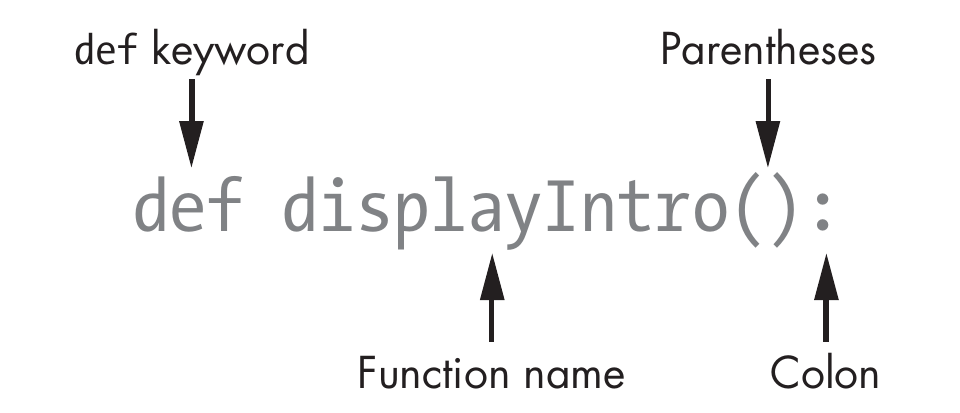
\includegraphics[height=2cm]{images/function_signature_example.png}
			\end{figure}
		\end{column}

		\begin{column}{6cm}
            \begin{lstlisting}
def displayIntro():
    print('''Ti trovi in una terra piena di draghi...''')
    print()
            \end{lstlisting}
		\end{column}
	\end{columns}
	! notiamo il print(''' '''), stringa multilinea
\end{frame}

\begin{frame}
\frametitle{Funzioni}
    \begin{block}{Alcuni consigli..}
        \begin{itemize}
            \item Ciò che abbiamo detto per i nomi delle variabili vale anche per i nomi delle funzioni
            \item Meglio se le nostre funzioni sono corte, con poco codice
            \item  Con 1 funzione facciamo 1 cosa soltanto!
            \item Evitiamo di usare più di 1 o 2 parametri in una funzione

            Se abbiamo bisogno di più parametri dividiamo quello che vogliamo fare in più funzioni
        \end{itemize}
    \end{block}
\end{frame}

\begin{frame}[fragile]
\frametitle{Funzioni}
    \begin{block}{Funzioni con parametri}
        \begin{itemize}
            \item Possiamo "dare in pasto" ad una funzione dei dati, delle informazioni, che chiamiamo \textbf{parametri}
            \item Queste informazioni ci serviranno per elaborare il risultato della funzione
        \end{itemize}
    \end{block}

    \begin{lstlisting}
                          # O ancora meglio..
def isPositive(number): | def isPositive(number):
    if number > 0 :     |    return number > 0
        return True     |
    else:               |
        return False    |
    \end{lstlisting}

    \begin{lstlisting}
# Usiamo la funzione, ad esempio, in questo modo
print(isPositive(5))    # True
print(isPositive(-5))   # False
    \end{lstlisting}

\end{frame}

\begin{frame}[fragile]
\frametitle{Funzioni}
    \begin{block}{Funzioni con parametri}
        \begin{itemize}
            \item Possiamo "dare in pasto" ad una funzione dei dati, delle informazioni, che chiamiamo \textbf{parametri}
            \item Queste informazioni ci serviranno per elaborare il risultato della funzione
            \item Il risultato verrà restituito utilizzando la keyword \textbf{return}
        \end{itemize}
    \end{block}

    \begin{lstlisting}
def sum(firstNumber, secondNumber):
    return firstNumber + secondNumber
    \end{lstlisting}

    \begin{lstlisting}
# Usiamo la funzione, ad esempio, in questo modo
result = sum(5, 4)    # result avra' valore 9
result = sum(-10, 5)  # result avra' valore -5
    \end{lstlisting}

\end{frame}
